\documentclass{beamer}
\mode<presentation> {\usetheme{Madrid}}

\definecolor{VIOLET}{rgb}{0.32549, 0.25098, 0.35294}
\definecolor{DARK}{rgb}{0.0, 0.0, 0.0}
\usecolortheme[named=DARK]{structure}

\usepackage{graphicx}
\usepackage{booktabs}
\usepackage{listings}
\usepackage[vietnamese]{babel}
\usepackage{xcolor}
\usepackage{hyperref}
\usepackage[labelformat=empty]{caption}
\usepackage{listings}
\lstset{language=Java,
        basicstyle=\footnotesize\ttfamily,
        keywordstyle=\footnotesize\color{blue}\ttfamily}

\title[Phát triển phần mềm cho thiết bị di động]{Clover - Ứng dụng mua sắm thời trang}
\author{\textbf{Nhóm 09}}
\institute[] {
    \begin{flushleft}
        \textbf{Thành viên}
        \begin{itemize}
            \item 20424008 - Dương Mạnh Cường (nhóm trưởng)
            \item 19424015 - Dương Trọng Đức
            \item 20424013 - Phạm Nguyễn Mỹ Diễm
        \end{itemize}
    \end{flushleft}

    \medskip
    \begin{figure}[h]
        \centering
\includegraphics[width=1.5cm]{images/logo.png}
    \end{figure}
    \textit{Đại học Khoa Học Tự Nhiên\\ĐHQG Thành phố Hồ Chí Minh} % 
}
\date{\tiny{05/01/2022}} 


\begin{document}

% ==========================================================================Title part
\begin{frame}
    \titlepage
\end{frame}


% =================================================================== Table of content
\begin{frame}
    \frametitle{Nội dung}
    \tableofcontents
\end{frame}

% ======================================================== Detail for table of content
\section{Giới thiệu về ứng dụng Clover}

\section{Các package + dịch vụ bên thứ ba}
\subsection{Các package}
\subsection{Các dịch vụ bên thứ ba}

\section{Các màn hình và chức năng kèm theo + mã nguồn}

\section{Chạy thử ứng dụng}

\section{Tài nguyên và tham khảo}

\section{Hỏi đáp và kết thúc}

% ============================================================================ Slide 3
\begin{frame}
    \frametitle{Giới thiệu về ứng dụng Clover}
    \begin{columns}
        \column{0.3\linewidth}
        \begin{figure}
            \centering
            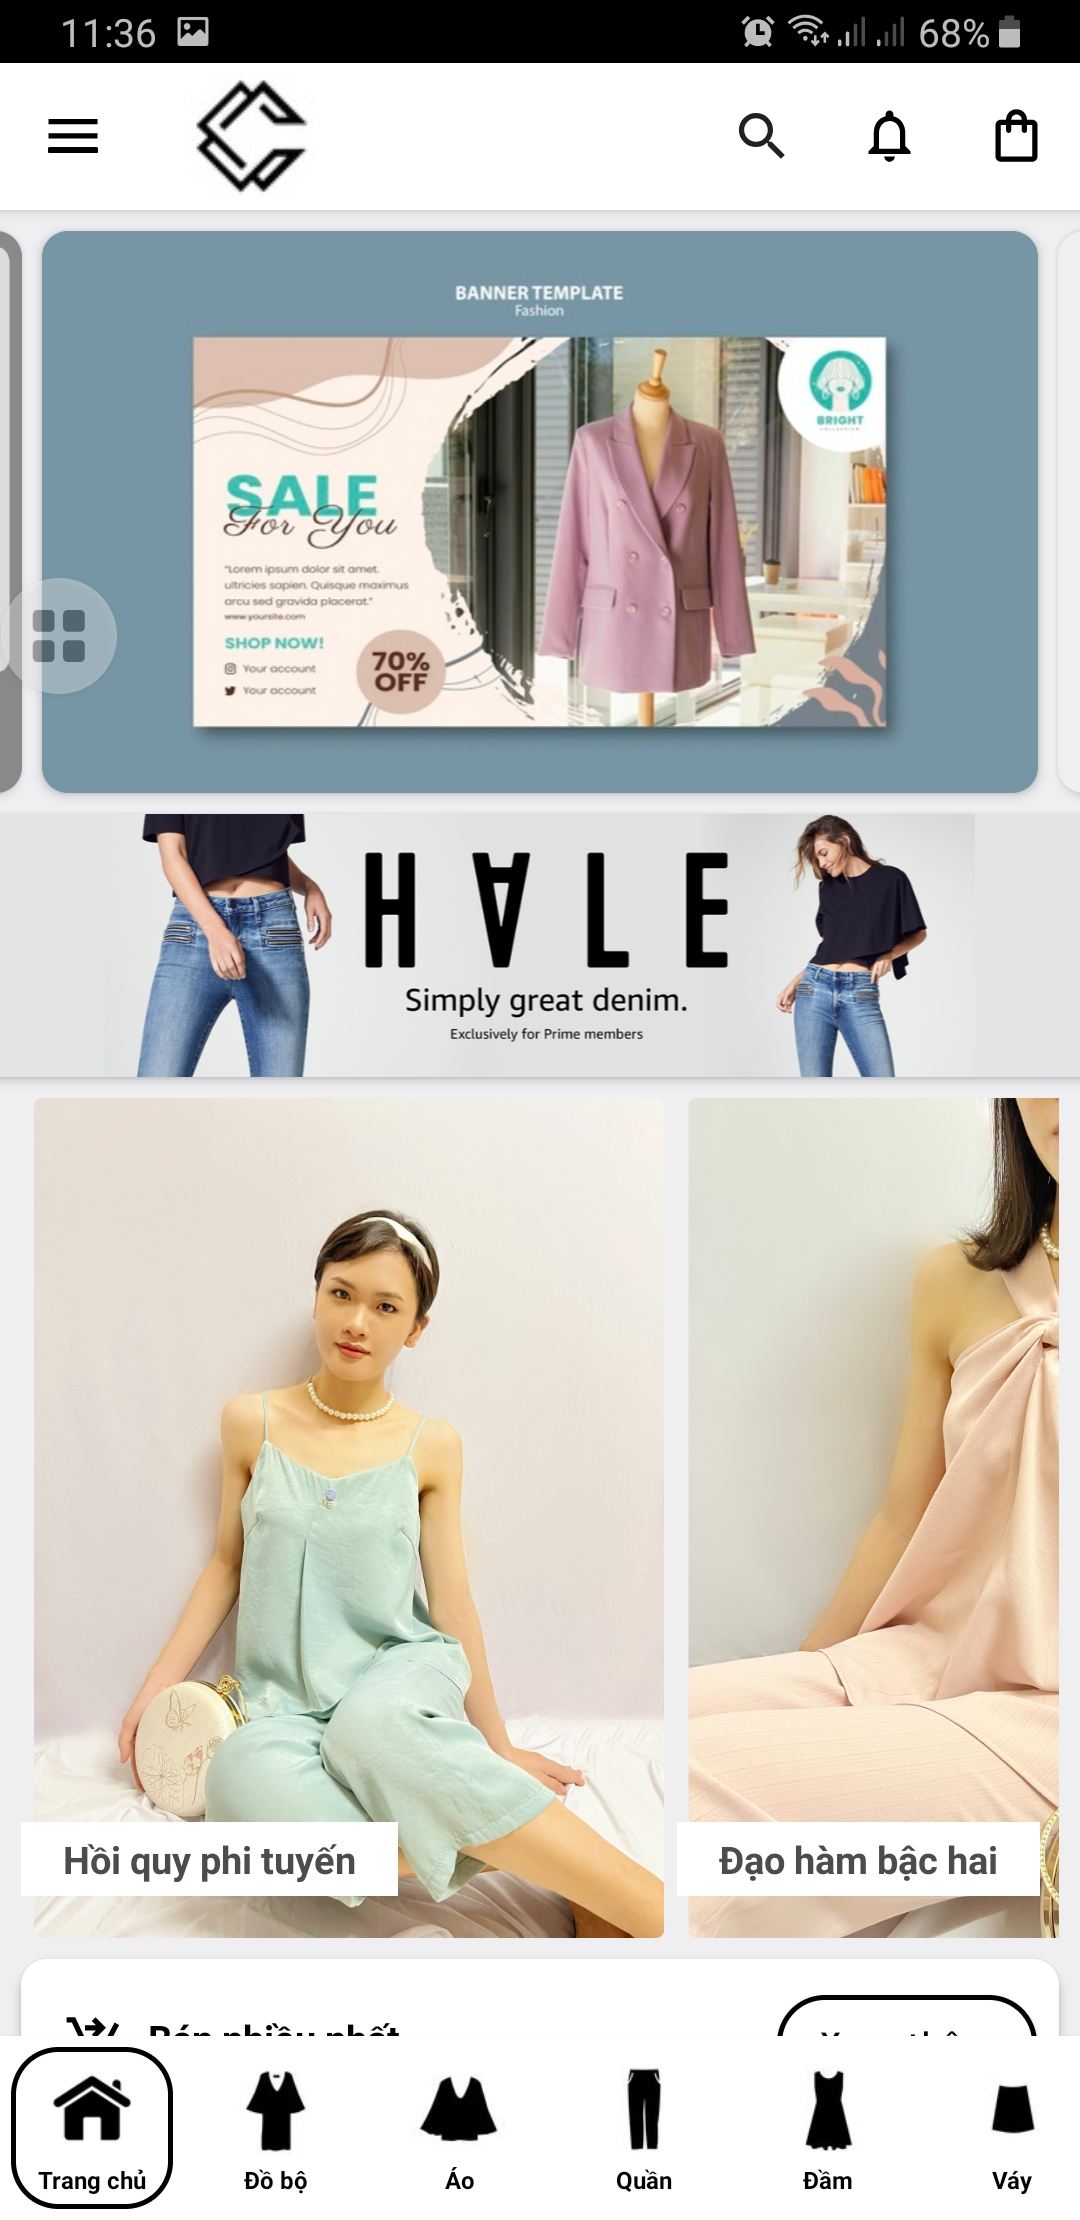
\includegraphics[height=0.7\textheight]{images/01.png}
            \caption{\centering\tiny{Hình 1: Màn hình chính của ứng dụng sau khi đăng nhập}}

        \end{figure}
        \column{0.7\linewidth}
        \begin{itemize}
            \item Clover \textbf{không phải} là một e-commerce mobile application.
            \item Clover là một \textbf{fashion mobile application} phục vụ cho các nhãn hàng thời trang mà họ không muốn kinh doanh sản phẩm của mình trên các trang thương mại điện tử.
            \item Các fashion mobile application khác mà Clover có tính năng tương tự: \href{https://play.google.com/store/apps/details?id=com.coupletx&hl=vi&gl=US}{\color{blue} CoupleTX}, \href{https://play.google.com/store/apps/details?id=vn.mrsimple&hl=en&gl=US}{\color{blue} Mr.Simple}, \href{https://play.google.com/store/apps/details?id=com.peekcloppenburg.mobileshop&hl=en&gl=US}{\color{blue} Peek \& Cloppenburg}, \href{https://play.google.com/store/apps/details?id=com.farfetch.farfetchshop&hl=en&gl=US}{\color{blue} Farfetch},...

            \item Hạn chế của ứng dụng đến hiện tại:
                  \begin{itemize}
                      \item Chưa có server.
                      \item Chưa có các web service.
                      \item Một vài chức năng còn sơ sài và chưa khớp với thực tế.
                      \item ...
                  \end{itemize}
        \end{itemize}
    \end{columns}
\end{frame}

% ============================================================================ Slide 4
\begin{frame}
    \frametitle{Các package + dịch vụ bên thứ ba (1)}
    \begin{flushleft}
        \large{\textbf{Các package:}}
        \begin{itemize}
            \item \textnormal{\href{https://github.com/vinc3m1/RoundedImageView}{\color{blue} \texttt{RoundedImageView}} - Tạo ra các \texttt{ImageView} bo tròn ở các góc, import vào gradle:}\\\texttt{\scriptsize{implementation 'com.makeramen:roundedimageview:2.3.0'}}

            \item \textnormal{\href{https://github.com/bumptech/glide}{\color{blue} \texttt{Glide}} - Load ảnh từ internet vào \texttt{ImageView}, import vào gradle:}\\\texttt{\scriptsize{implementation 'com.github.bumptech.glide:glide:4.12.0'\\annotationProcessor 'com.github.bumptech.glide:compiler:4.12.0'}}

            \item Và một vài package khác.
        \end{itemize}
    \end{flushleft}
\end{frame}

% ============================================================================ Slide 5
\begin{frame}
    \frametitle{Các package + dịch vụ bên thứ ba (2)}
    \begin{flushleft}
        \large{\textbf{Các dịch vụ bên thứ ba:}}
        \begin{itemize}
            \item \textnormal{\href{https://firebase.google.com/docs/firestore/quickstart}{\color{blue} \textsf{Firebase Firestore}} - CSDL NoSQL do Google phát triển.}

            \item \textnormal{Firebase FireStorage - Dùng để lưu trữ tệp tin, thư mục trên cloud, nhóm không tìm thấy document do Google công bố cho dịch vụ này, nhưng để sử dụng thì nhóm tìm hiểu trong cuốn} \href{https://www.amazon.com/Mastering-Firebase-Android-Development-cloud-enabled/dp/1788624718}{\color{teal} Mastering Firebase for Android Development}.

            \item \textnormal{\href{https://firebase.google.com/docs/auth/android/start}{\color{blue} \textsf{Firebase Authentication}} - Dịch vụ xác nhận danh tính, đăng ký tài khoản người dùng do Google phát triển.}
        \end{itemize}
    \end{flushleft}
\end{frame}

% ============================================================================ Slide 6
\begin{frame}
    \frametitle{Các màn hình và chức năng kèm theo + mã nguồn (1)}
    \framesubtitle{Nội dung}
    \begin{flushleft}
        \large{\textbf{Trình bày: } 19424013 - Dương Trọng Đức}
        \begin{itemize}
            \item Màn hình + chức năng đăng nhập.
        \end{itemize}
    \end{flushleft}

    \begin{flushleft}
        \large{\textbf{Trình bày: } 20424013 - Phạm Nguyễn Mỹ Diễm}
        \begin{itemize}
            \item Màn hình chi tiết sản phẩm và chức năng kèm theo.
        \end{itemize}
    \end{flushleft}

    \begin{flushleft}
        \large{\textbf{Trình bày: } 20424008 - Dương Mạnh Cường}
        \begin{itemize}
            \item Màn hình chính của ứng dụng.
            \item Chức năng tìm kiếm.
        \end{itemize}
    \end{flushleft}

    \begin{flushleft}
        Ngoài ra còn có các màn hình khác như \textsf{\color{teal} Giỏ hàng, Lịch sử mua hàng, Tài khoản người dùng,...} nhưng đơn giản và không phức tạp bằng những màn hình + chức năng trên nên nhóm xin rút gọn phần trình bày cho chúng.
    \end{flushleft}
\end{frame}

% ============================================================================ Slide 7
\begin{frame}
    \frametitle{Các màn hình và chức năng kèm theo + mã nguồn (2)}
    \framesubtitle{Màn hình + chức năng đăng nhập}

    \begin{columns}
        \column{0.3\linewidth}
        \begin{figure}
            \centering
            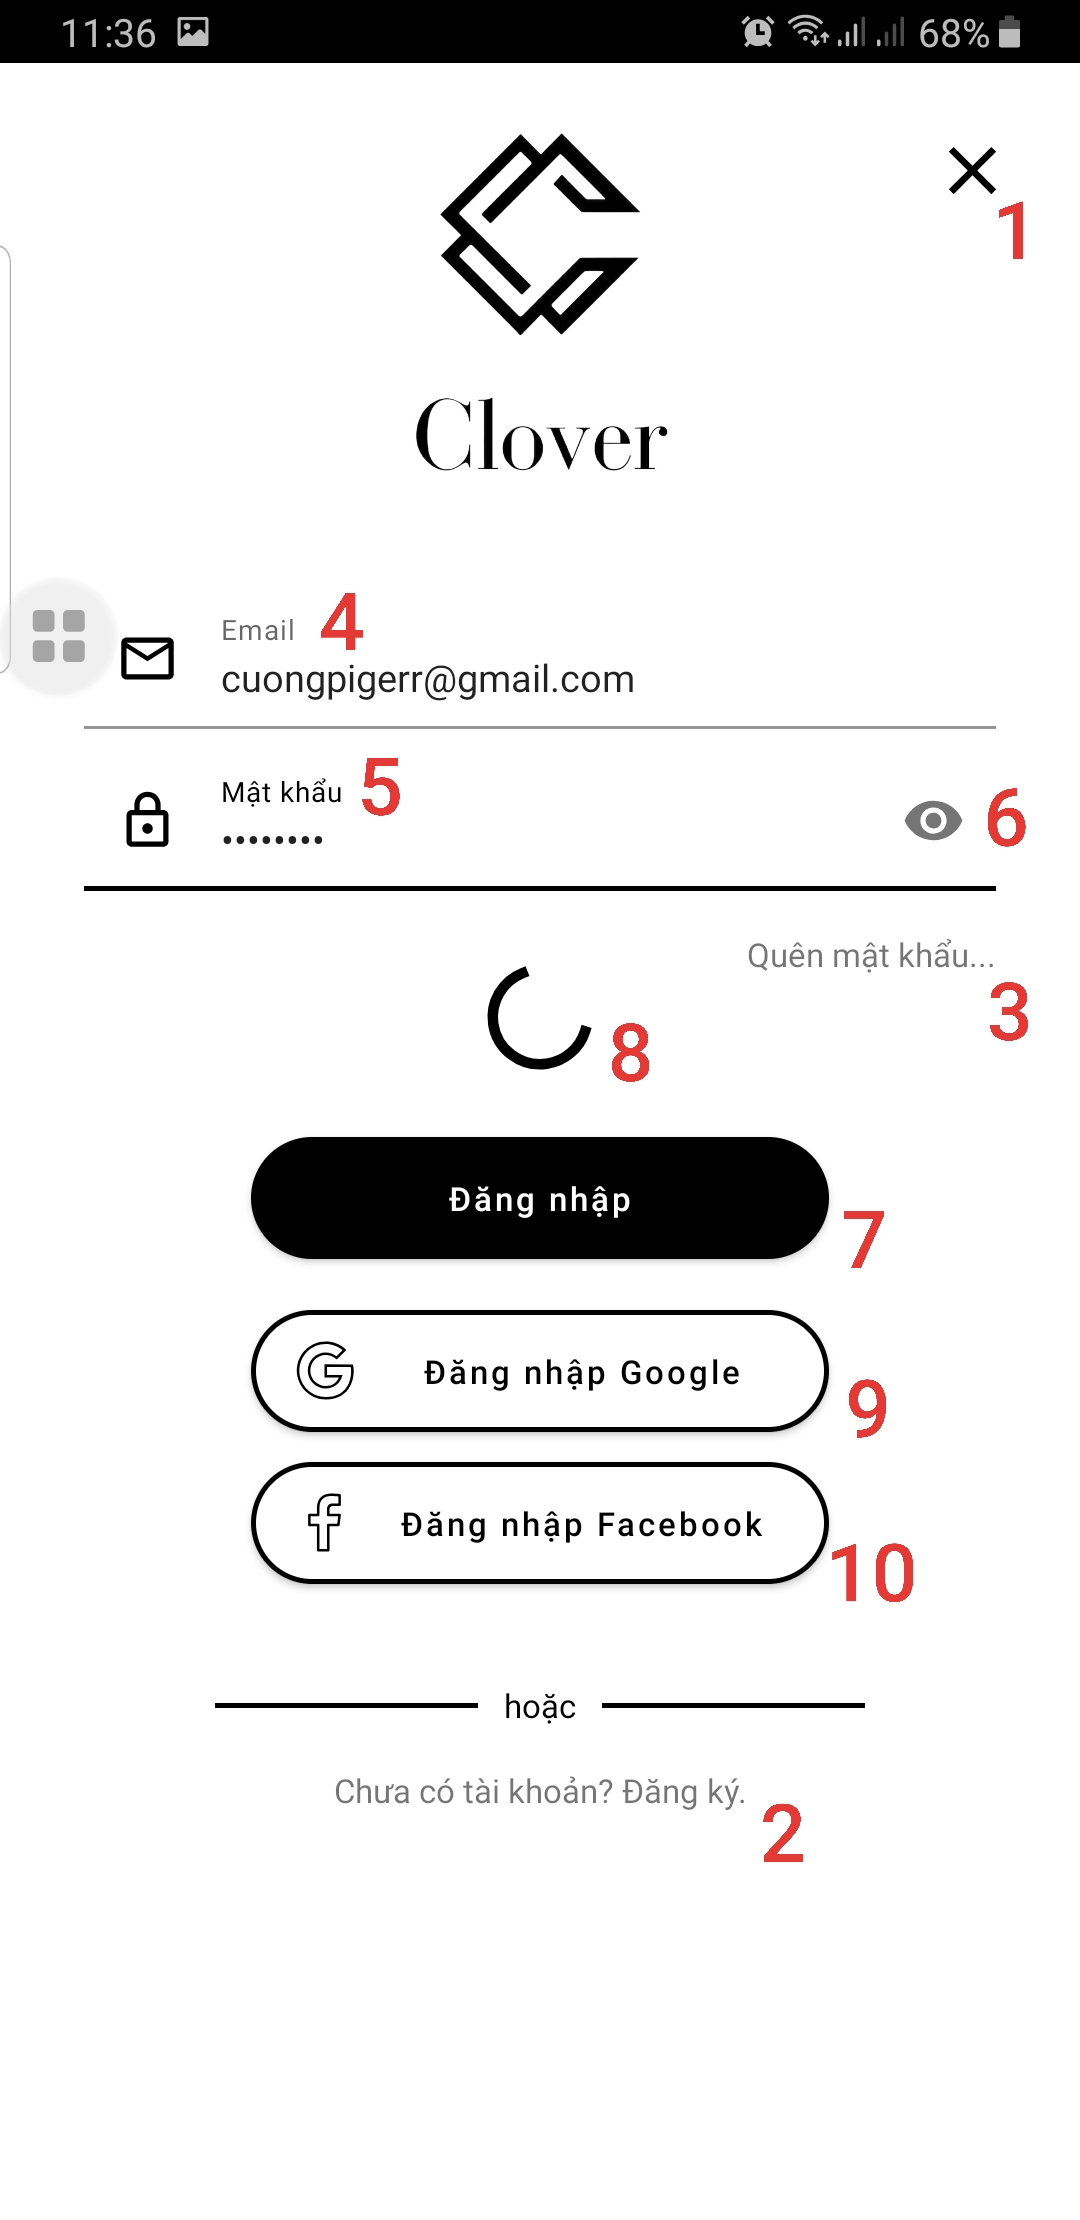
\includegraphics[height=0.7\textheight]{images/02.png}
            \caption{\centering\tiny{Hình 2: Màn hình đăng nhập}}

        \end{figure}
        \column{0.7\linewidth}
        \indent \textbf{Các thành phần và chức năng kèm theo trên màn hình:}
        \begin{itemize}
            \item \textbf{1}: Image button - khi nhấn vào button này người dùng sẽ được chuyển thẳng đến màn hình chính của ứng dụng mà \textbf{không cần đăng nhập}.
            \item \textbf{2}: Text button - khi nhấn vào sẽ đưa đến fragment đăng ký tài khoản mới cho người dùng.
            \item \textbf{3}: Text button - khi nhấn vào đưa người dùng đến fragment đặt lại mật khẩu.
            \item \textbf{4}: Text input layout - nhập thông tin email của người dùng.
        \end{itemize}
    \end{columns}
\end{frame}

% ============================================================================ Slide 8
\begin{frame}
    \begin{columns}
        \column{0.3\linewidth}
        \begin{figure}
            \centering
            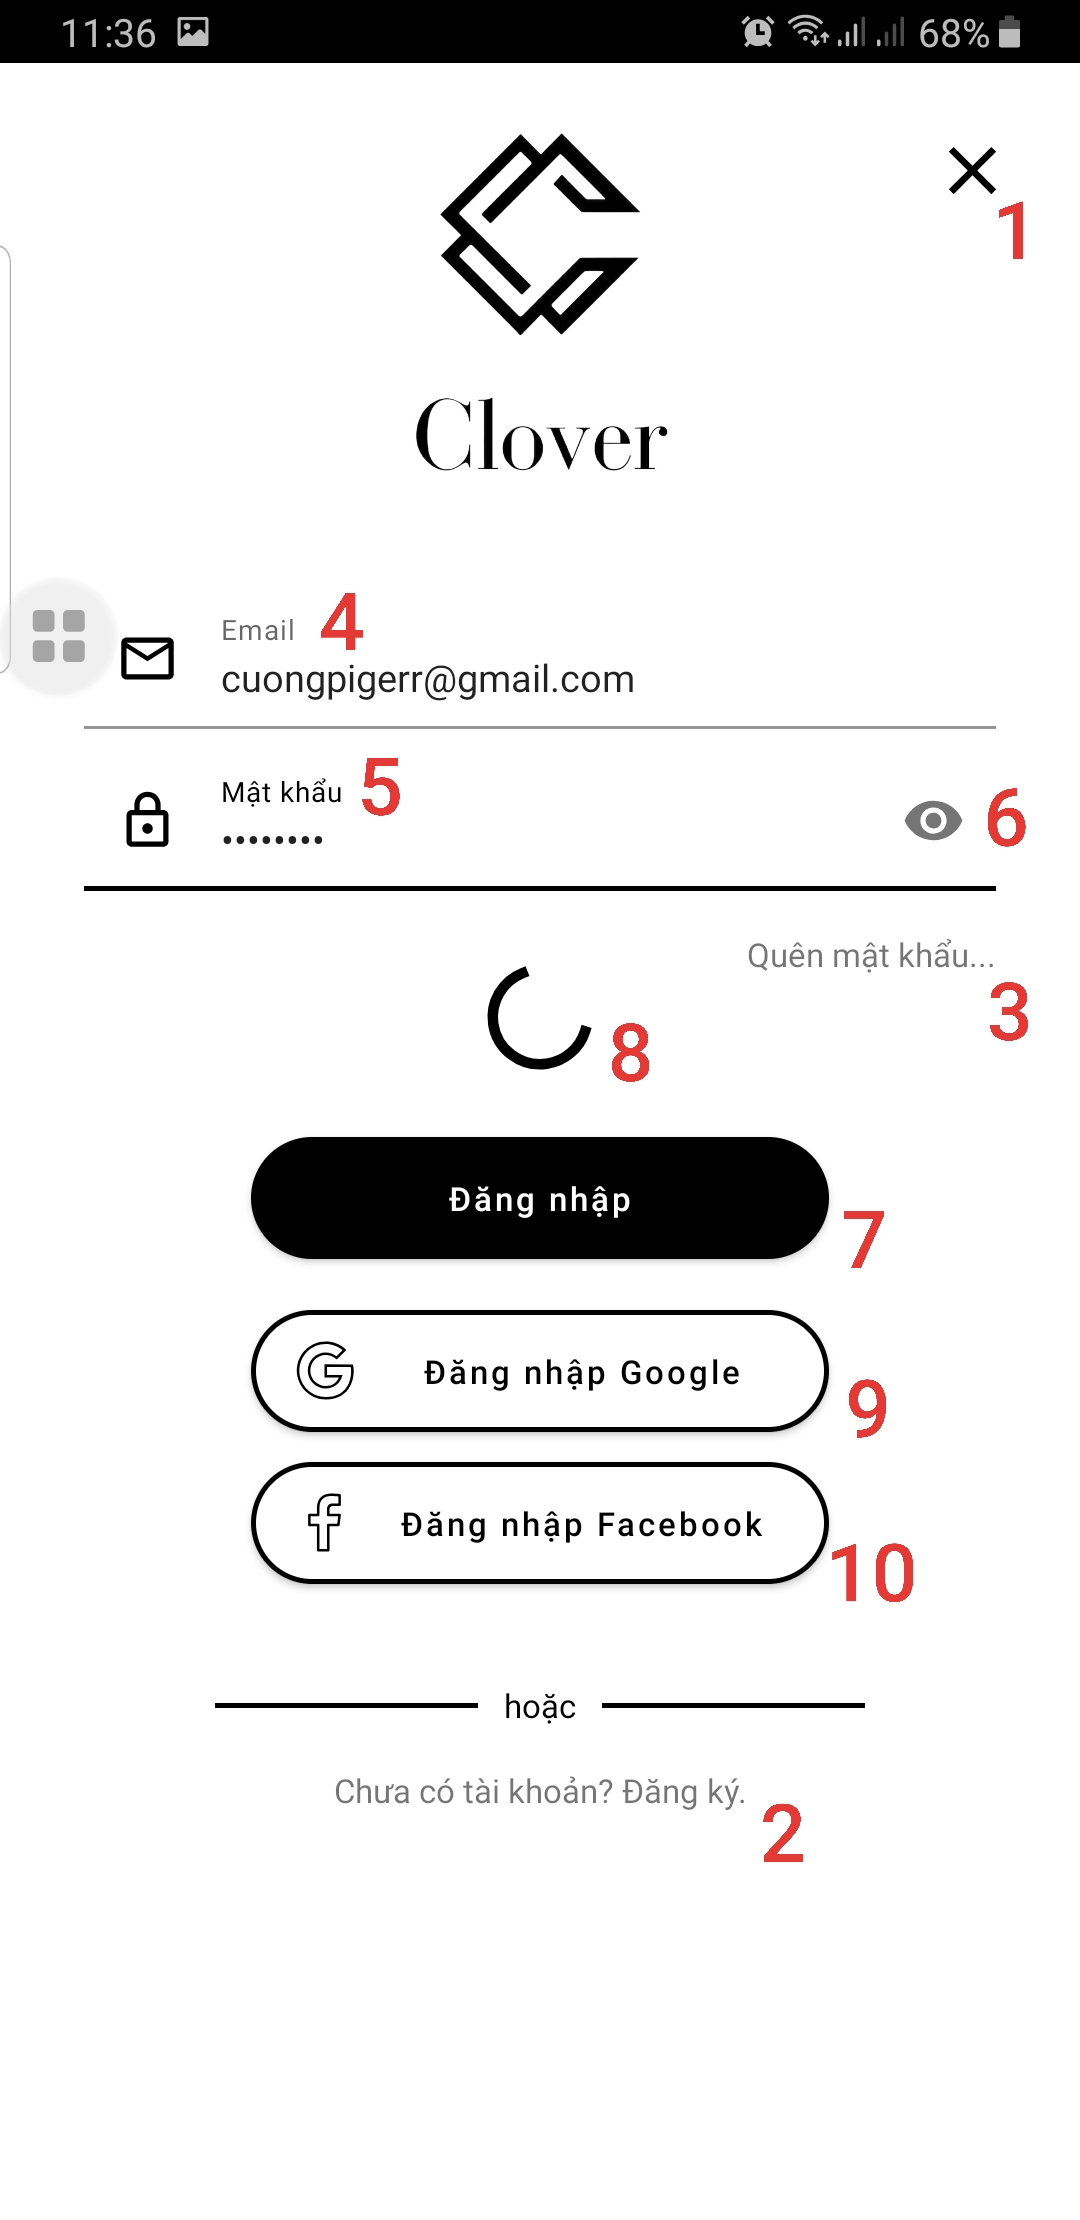
\includegraphics[height=0.7\textheight]{images/02.png}
            \caption{\centering\tiny{Hình 2: Màn hình đăng nhập}}

        \end{figure}
        \column{0.7\linewidth}
        \indent \textbf{Các thành phần và chức năng kèm theo trên màn hình:}
        \begin{itemize}
            \item \textbf{5}: Text input layout - nhập mật khẩu của người dùng.
            \item \textbf{6}: Icon - khi nhấn vào sẽ hiển thị mật khẩu ở \textbf{5} ra dưới dạng text.
            \item \textbf{7}: Button - nhấn vào để đăng nhập.
            \item \textbf{8}: Progress Circle - luôn ẩn đi, chỉ hiển thị khi người dùng nhấn vào \textbf{7} để cho người dùng biết rằng hệ thống vẫn chạy và đang trong quá trình kiểm tra đăng nhập.
        \end{itemize}

        \href{https://github.com/cuongpiger/Sharing/blob/main/Clover/SignInFragment.java}{\color{blue} Mã nguồn.}
    \end{columns}
\end{frame}

% ============================================================================ Slide 9
\begin{frame}
    \frametitle{Các màn hình và chức năng kèm theo + mã nguồn (3)}
    \framesubtitle{Màn hình chi tiết sản phẩm và chức năng kèm theo}

    \begin{columns}
        \column{0.3\linewidth}
        \begin{figure}
            \centering
            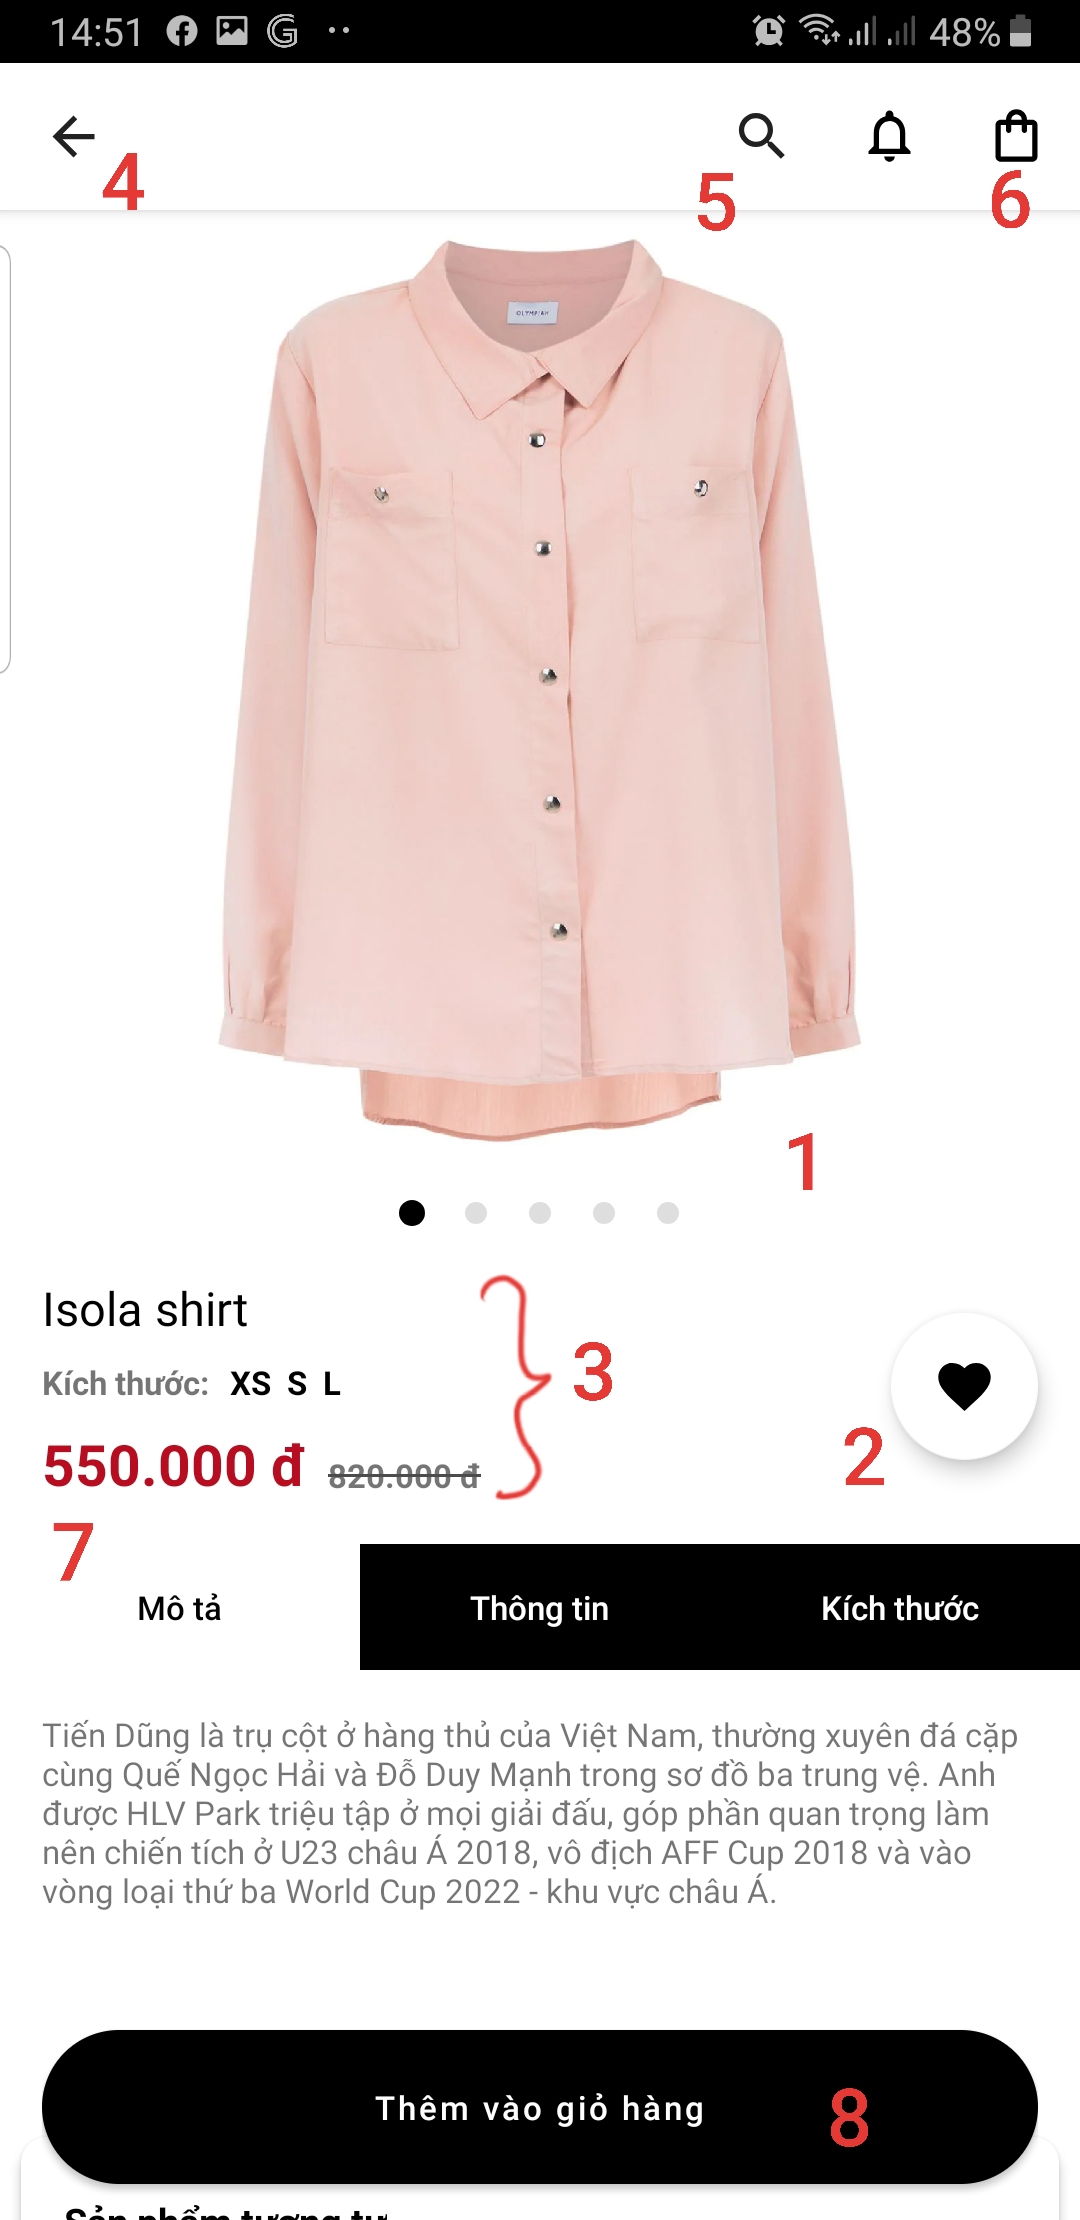
\includegraphics[height=0.7\textheight]{images/03.png}
            \caption{\centering\tiny{Hình 3: Màn hình chi tiết sản phẩm 1}}

        \end{figure}
        \column{0.7\linewidth}
        \indent \textbf{Các thành phần và chức năng kèm theo trên màn hình:}
        \begin{itemize}
            \item \textbf{1}: View Pager - hiển thị các hình ảnh của sản phẩm.
            \item \textbf{2}: Floating Action Button - cho phép người dùng nhấn vào để thêm sản phầm vào mục yêu thích.
            \item \textbf{3}: Các text view - hiển thị thông tin của sản phẩm.
            \item \textbf{4}: As home indicator - quay về fragment trước đó được lưu trong backstack.
        \end{itemize}
    \end{columns}
\end{frame}

% =========================================================================== Slide 10
\begin{frame}
    \begin{columns}
        \column{0.3\linewidth}
        \begin{figure}
            \centering
            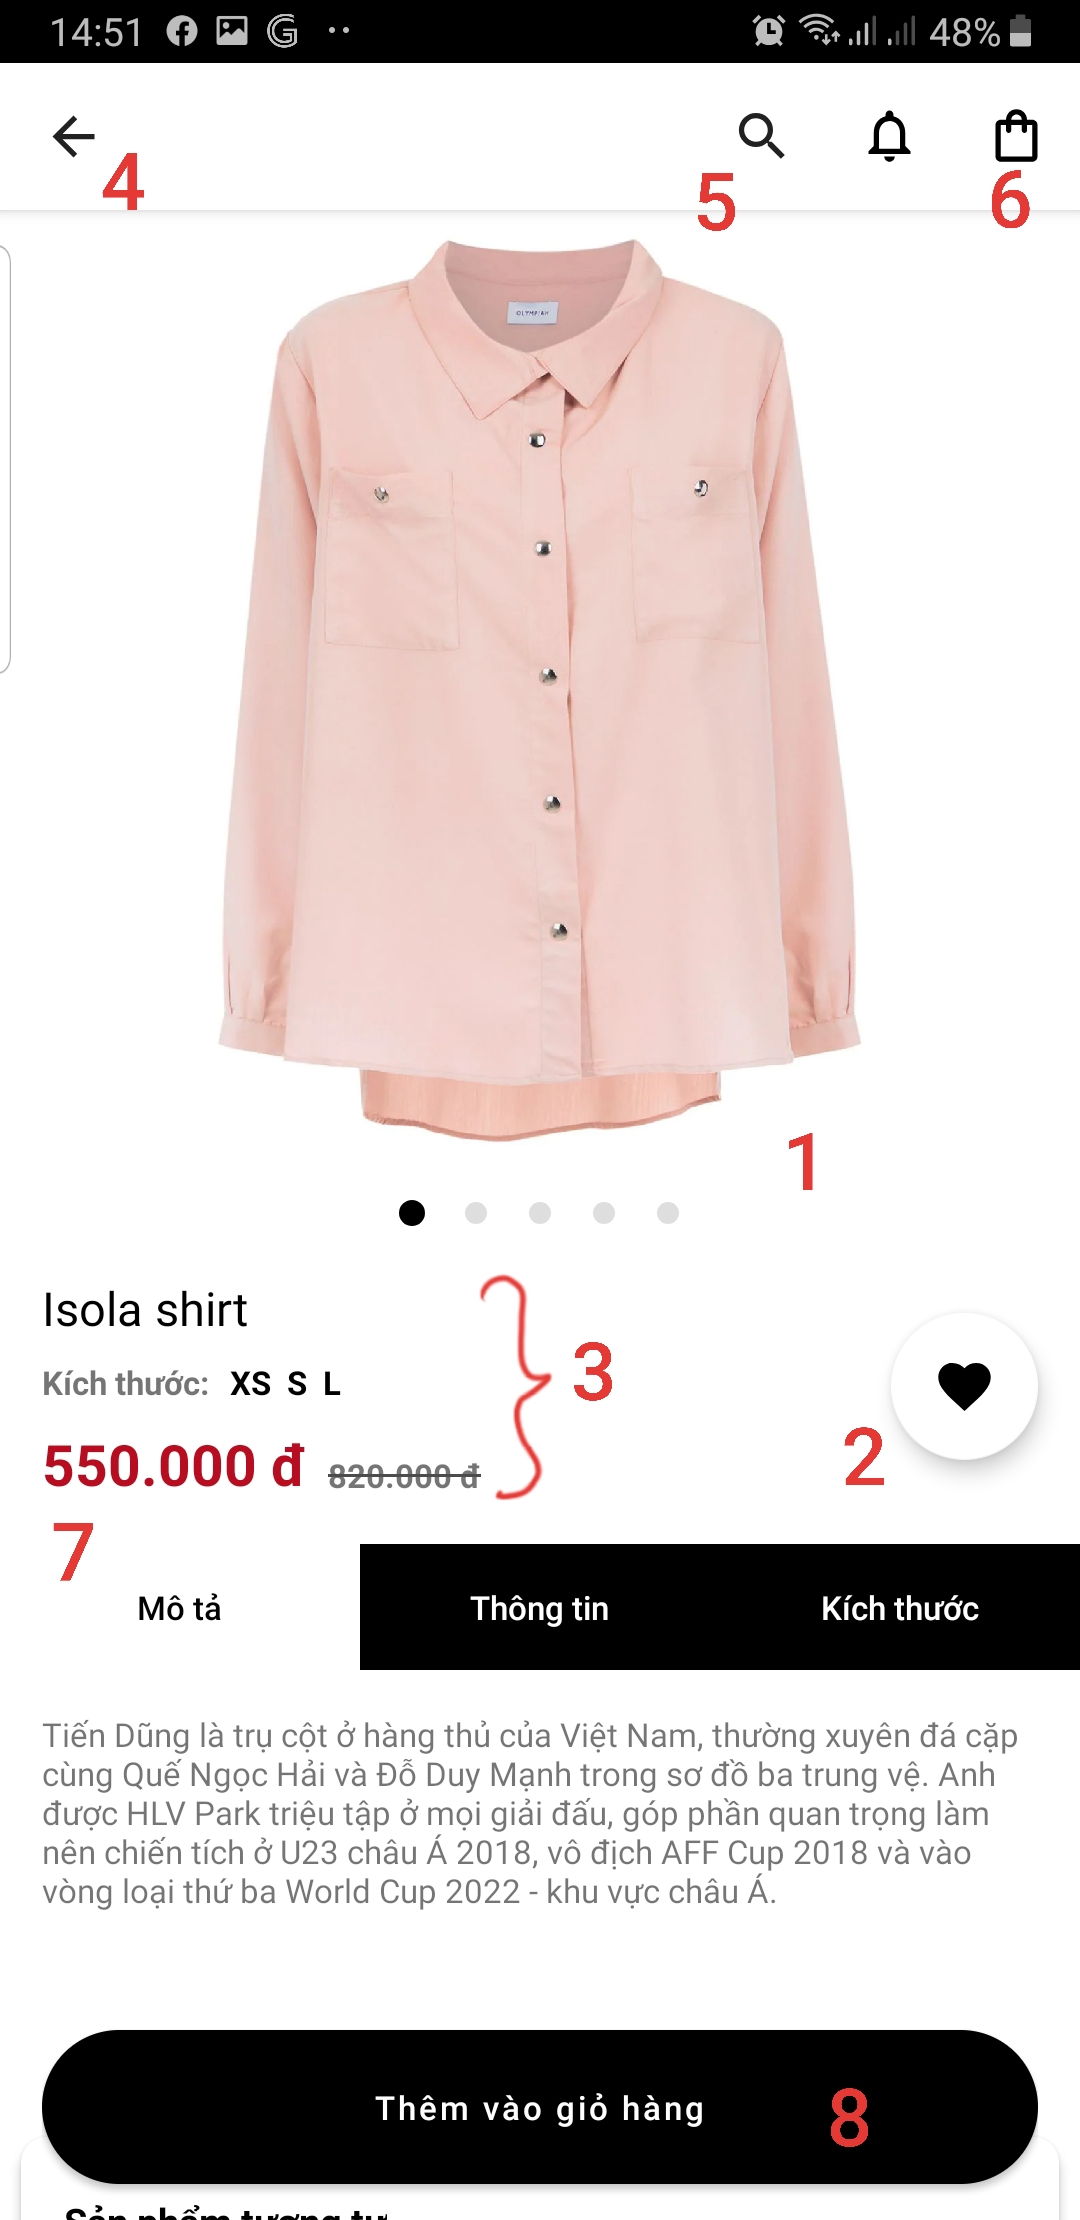
\includegraphics[height=0.7\textheight]{images/03.png}
            \caption{\centering\tiny{Hình 3: Màn hình chi tiết sản phẩm 1}}

        \end{figure}
        \column{0.7\linewidth}
        \indent \textbf{Các thành phần và chức năng kèm theo trên màn hình:}
        \begin{itemize}
            \item \textbf{5}: Menu item Search - nhấn vào để thực hiện chức năng tìm kiếm.
            \item \textbf{6}: Menu item Cart - nhấn vào để đến fragment giỏ hàng.
            \item \textbf{7}: TabLayout + View Pager 2 - hiển thị các thông tin thêm về sản phẩm. Bên trong tab "Mô tả" là một Text View, bên trong tab "Thông tin" và "Kích thước" là các GridView.
            \item \textbf{8}: Button - nhấn vào sẽ hiện một Dialog để người dùng có thể chọn size và số lượng sản phẩm để thêm vào giỏ hàng.     
        \end{itemize}
    \end{columns}
\end{frame}

% =========================================================================== Slide 11
\begin{frame}
    \begin{columns}
        \column{0.3\linewidth}
        \begin{figure}
            \centering
            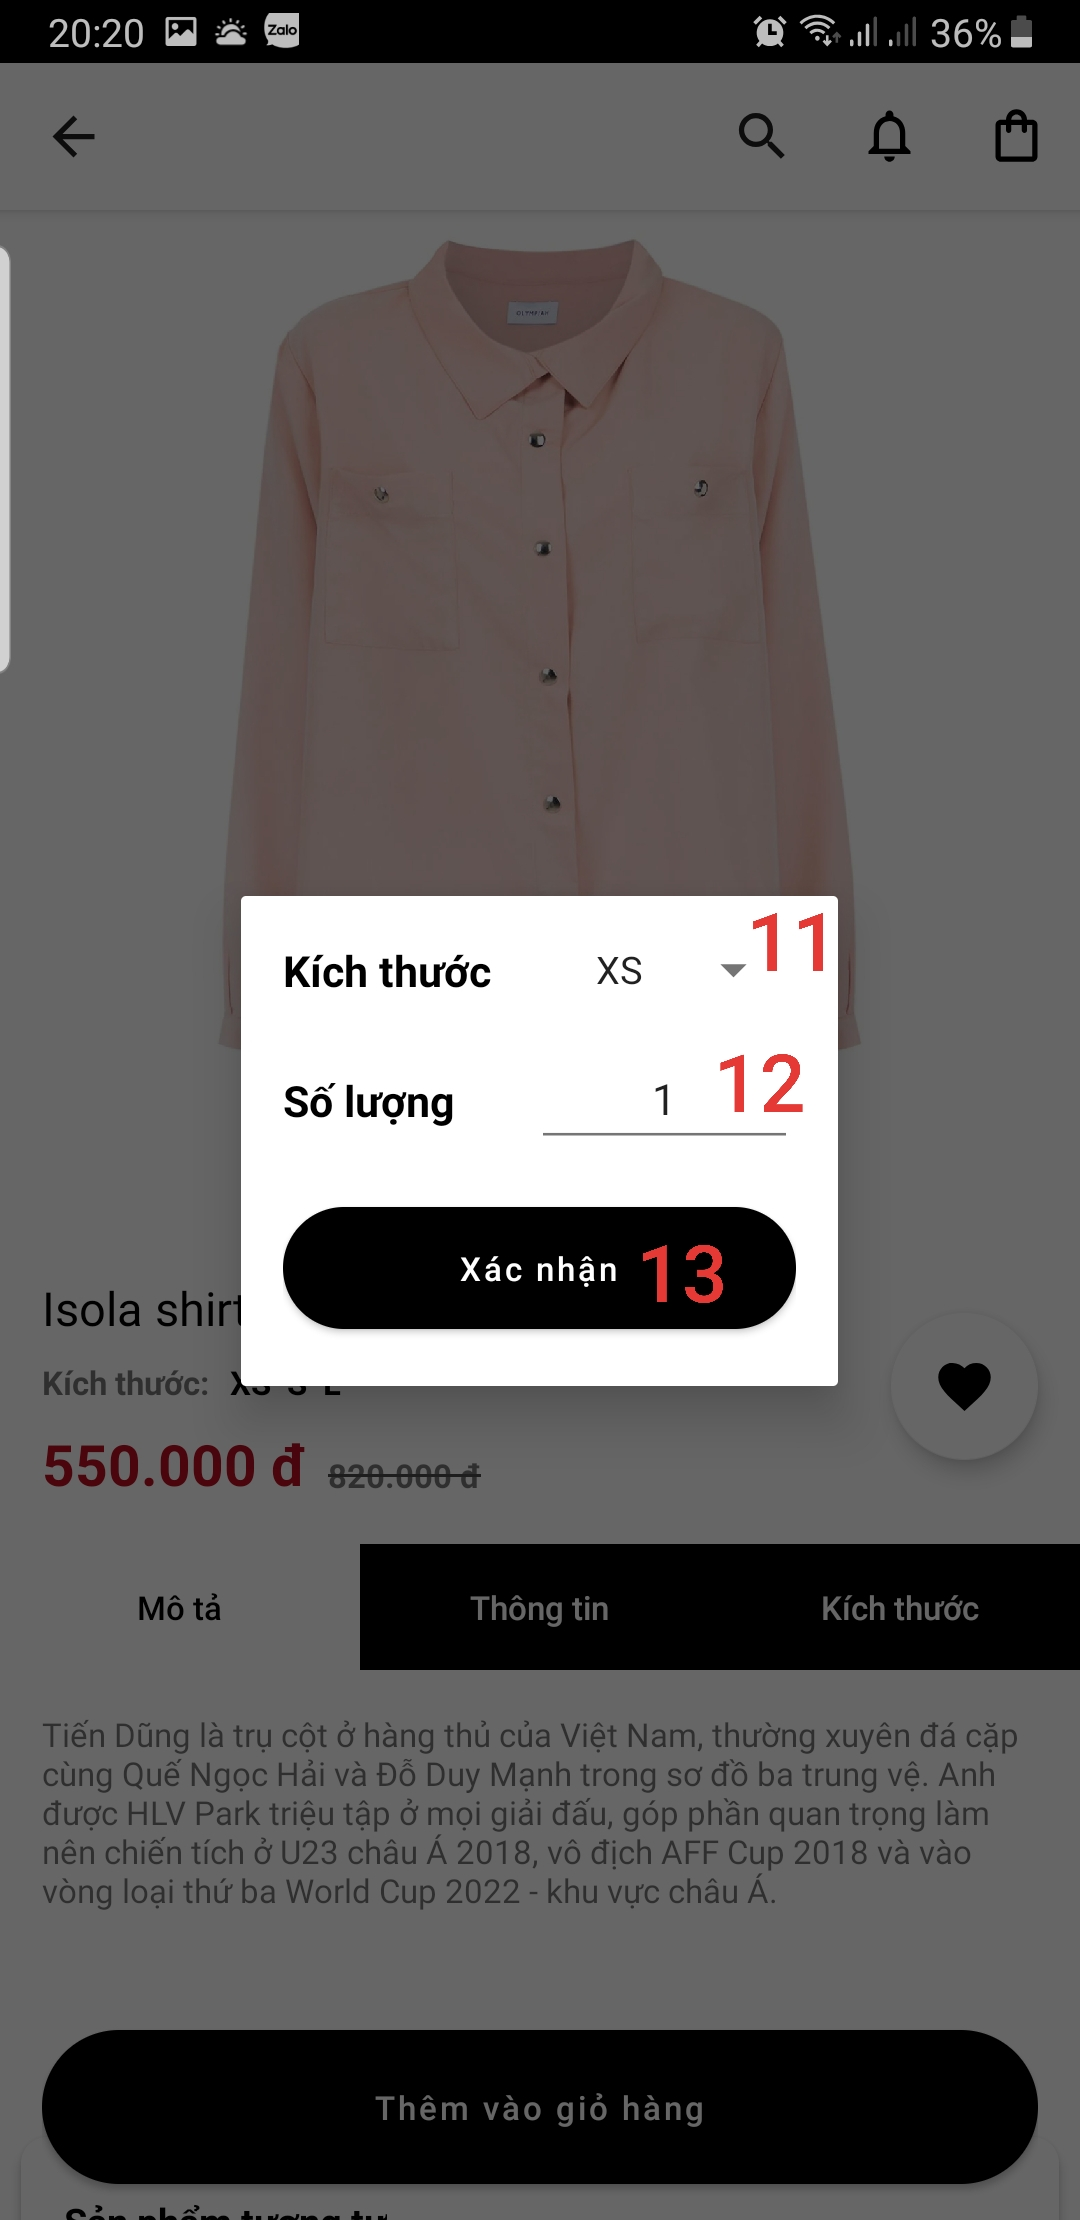
\includegraphics[height=0.7\textheight]{images/04.png}
            \caption{\centering\tiny{Hình 4: Màn hình chi tiết sản phẩm 2}}

        \end{figure}
        \column{0.7\linewidth}
        \indent \textbf{Các thành phần và chức năng kèm theo trên màn hình:}
        \begin{itemize}
            \item \textbf{11}: Spinner - cho phép người dùng chọn các size của sản phẩm.
            \item \textbf{12}: Text input - để người dùng nhập số lượng sản phẩm cần mua cho size tương ứng.
            \item \textbf{13}: Button - khi click vào sản phẩm sẽ được thêm vào giỏ hàng cùng size và số lượng đã chọn.         
        \end{itemize}

        \href{https://github.com/cuongpiger/Sharing/blob/main/Clover/SignInFragment.java}{\color{blue} Mã nguồn 1 - View Pager.}

        \href{https://github.com/cuongpiger/Sharing/blob/main/Clover/SignInFragment.java}{\color{blue} Mã nguồn 2 - Thêm sản phẩm vào giỏ hàng.}
    \end{columns}
\end{frame}

\begin{frame}
    \frametitle{}
    \begin{block}{ - Mối đe dọa từ chối và phá hủy}

        \begin{itemize}
            \item Các mối đe dọa từ chối hoặc phá hủy làm cho tài sản hoặc tài nguyên không có sẵn hoặc không thể sử dụng được.
            \item Vi phạm nguyên lý sẵn có của bảo mật thông tin.
            \item Một cuộc tấn công từ chối hoặc phá hủy thành công khi nó ngăn người dùng được ủy quyền truy cập tài nguyên tạm thời hoặc vĩnh viễn.
            \item Tấn công DoS là một ví dụ về mối đe dọa từ chối hoặc phá hủy.
        \end{itemize}
    \end{block}
\end{frame}

%------------------------------------------------

\begin{frame}
    \frametitle{Tấn công khai thác lỗ hổng}

    \textbf{Các cuộc tấn công có thể bao gồm cả 4 phương thức sau:}
    \begin{enumerate}
        \item Giả mạo: tạo ra một số mánh khóe để người dùng không nghi ngờ hệ thống đã bị tấn công.
        \item Chặn thông tin: Liên quan đến việc nghe lén các truyền và chuyển hướng chúng để sử dụng trái phép.
        \item Gián đoạn thông tin: Gây ra sự gián đoạn trong một kênh truyền thông, ngăn chặn việc truyền dữ liệu.
        \item Thay đổi thông tin: thay đổi dữ liệu có trong các đường truyền hoặc tập tin.
    \end{enumerate}

    \textbf{2 nhóm tấn công:}
    \begin{enumerate}
        \item Tấn công nhằm thay đổi các dữ liệu.
        \item Tấn công nhằm nghe lén và theo dõi các dữ liệu.
    \end{enumerate}
\end{frame}
%------------------------------------------------
\begin{frame}
    \frametitle{Các tấn công độc hại}
    \begin{block}{Birthday attacks:}
        \begin{itemize}
            \item Tấn công Ngày sinh là một loại tấn công mật mã dựa trên sự khai thác vấn đề Ngày sinh (Birthday problem)- một hiện tượng xác suất tạo ra nghịch lý đối với cảm giác của con người, do vậy còn được gọi là “Nghịch lý Ngày sinh”(Birthday paradox). Áp dụng lí thuyết xác suất thống kê, giả sử trong 1 phòng có 23 người ngẫu nhiên, xác suất có ít nhất  2 người trùng ngày sinh là 50\%.
            \item Công thức tổng quát để tính xác suất có ít nhất 2 người trùng ngày sinh trong n người ngẫu nhiên:
                  \begin{figure}[h]
                      \centering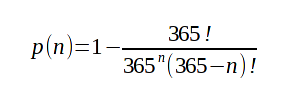
\includegraphics[width=0.4\linewidth]{images/bday.png}
                  \end{figure}
            \item Với n = 70 người ngẫu nhiên, p(n) ~ 99\%, nghĩa là gần như chắc chắn trong 70 người ngẫu nhiên có 2 người trùng ngày sinh.
        \end{itemize}
    \end{block}
\end{frame}


\begin{frame}
    \frametitle{Eavesdropping}
    \begin{block}{}
        Tạo ra các gói tin có địa chỉ IP giả mạo không là địa chỉ máy gửi gói tin
    \end{block}
    \begin{block}{}
        Vượt qua các kiểm soát về nguồn gốc địa chỉ IP.
    \end{block}
    \begin{block}{}
        Phục vụ các mô hình tấn công khác.
        \begin{itemize}
            \item Tấn công về phiên Tấn công về session.
            \item Tấn công kiểu phản xạ.
        \end{itemize}
    \end{block}
    \begin{block}{}
        Giải pháp:
        \begin{itemize}
            \item Không sử dụng xác thực là địa chỉ IP.
            \item Phát hiện các bất thường về kết nối Phát hiện các bất thường về kết nối mạng.
        \end{itemize}
    \end{block}
\end{frame}


\begin{frame}
    \frametitle{Hỏi đáp và kết thúc}
    
\includegraphics[width=\textwidth]{images/ask_and_answer.jpg}
\end{frame}




\begin{frame}
    \Huge{\centerline{HẾT}}
    \Large{\centerline{Cảm ơn Thầy và các bạn đã chú ý lắng nghe.}}
\end{frame}

%----------------------------------------------------------------------------------------

\end{document}